\documentclass[11pt, twocolumn]{article}

% GRAPHICS
\usepackage{float}
\usepackage{graphicx}
\usepackage{subcaption}

% HYPERLINKS
\usepackage{hyperref}

% DOCUMENT PADDING AND MARGINS
\usepackage{titlesec}
\usepackage[margin=0.8in]{geometry}
%\setlength{\parskip}{\baselineskip}%
%\setlength{\parindent}{0pt}
\titlespacing*{\section}{0pt}{2ex}{0ex}
\titlespacing*{\subsection}{0pt}{2ex}{0ex}
\titlespacing*{\subsubsection}{0pt}{2ex}{0ex}

%COMMENTING
\usepackage{comment}


\begin{document}

% TITLE
\title{Autonomous Quadrotor Landing on a Moving Platform}
\author{Stan Brown \& Chris Choi}
\date{}
\maketitle


\section{Introduction}
Autonomous 	precision landing of a quadrotor onto moving platform has been explored by a number of researchers \cite{Lee2012, Kim2014, Voos2010, Friis2009, Ling2014, Herisse2012}, and there exists a wide range of approaches to the problem. Possible applications for this work include autonomous landing on a boat in high wind conditions, landing on a charging platform and more.

The major challenge with autnomous precision landing is the difficulty of obtaining a reliable estimate of the landing target relative to the quadrotor, the landing target can often go out of the camera's field of view causing the quadrotor to lose track of the target, other vision based artifacts include lighting, and color.


\section{Related Work}
The challenging of autonoums landing can be categorized into three distinct parts. First, it must sense or detect the landing target to obtain positional estimates relative to the quadrotor. Secondly, the quadrotor must plan its rendezvous trajectory with the landing target. Third and finally, the quadrotor must apply a set of controller commands to approach the platform, matching both speed and heading on the approach and land on the moving target. We discuss the three different parts in the following subsections.

\subsection{Perception and State Estimation}
For perception existing solutions use a variety of simple to complex techniques. In  \cite{Kim2014} a basic color threshold technique was to identify the landing target, while \cite{Herisse2012} used optical flow in images captured on board the quadrotor to obtain necessary relative information for control. 

\subsection{Planning}
In the literature we reviewed, rendezvous planning was neglected as it was assumed that quadrotor has a clear view of its landing target. Most authors tend to focus on the detection and estimation of the quadrotor's pose relative to the target and maintaining an accurate estimation throughout the landing procedure which is mostly handled by a series of control loops.

\subsection{Control}
A comparison between a PID and Linear Quadratic Control (LQC) was explored in \cite{Friis2009}. However the authors admit, even though LQC performed slightly better than the PID controller the difference was minor and may be attributed to the additional time spent tuning the LQC. In \cite{Herisse2012} a PID controller was developed to land on a oscillating platform in the vertical direction with no lateral movement. While interesting, the solution took over 1 minute to transition from hovering over the landing pad to landing. Additionally the experiments did not seem to account for pitch or roll of the platform.  



\section{Proposed Methodology}
In reviewing prior work, a reoccurring problem lies in the difficulty in maintaining an accurate pose estimation between the quadrotor and the landing target throughout the entire manoeuvre. As the quadrotor approaches the landing target, the target often goes beyond the camera's field of view, causing camera based navigation techniques to fail. Furthermore, in certain conditions the tilt angle of the quadrotor could cause difficulty in maintaining a visual on the landing pad for a downward facing or fixed camera. 

To address both of these issues, we propose a novel solution utilizing an nested apriltags which we term inception apriltag. We will replicate the experiment performed by \cite{Ling2014}, where we assume the quadrotor already has a visual of the landing platform. We aim to implement a series of controllers for the approach and landing of the quadrotor to the moving landing platform.



\section{Project Progress}
\subsection{Hardware Setup}
\subsubsection{Quadrotor}
For the hardware, we have chosen to reuse equipment that is readily available to us in the Wave Lab. For the quadrotor we have been using the DJI F450 quadrotor frame, Emax 2213-935KV motors with complimentary 1045R propellers, Thunder Power lipo 11.1V 4200mah battery, DJI E310 420S 20A electronic speed controller and Pixhawk v2.4 as our flight controller.

\begin{figure}[H]
	\centering
	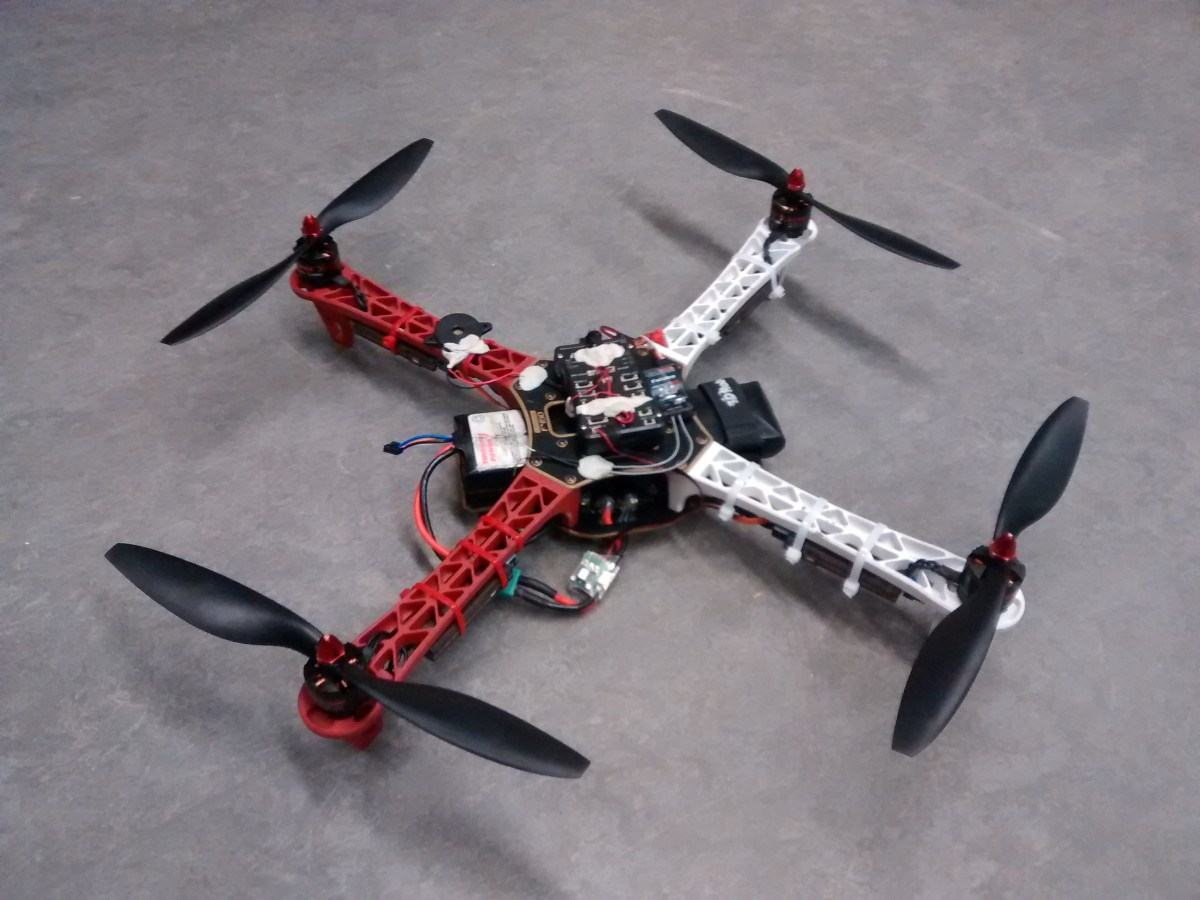
\includegraphics[width=0.8\linewidth]{images/quadrotor.jpg}
	\caption{DJI F450 with Pixhawk v1.5}
\end{figure}

\subsubsection{Onboard Autonomous Control System}
In terms of onboard autonoumos control, we have decided to use the Odriod XU4 due to its size and processing power available, and a Logitech C270 HD webcam as our vision sensor. One problem we may face very soon is the narrow field of view and relatively low frame rate (25Hz) the logitech webcam has. We will be keeping our options open, and plan on replacing the logitech webcam with a Ximia xiQ USB3 camera with a wide angle lens in the near future.



\subsection{Software Setup}
\subsubsection{Pixhawk Firmware - PX4}
As mentioned in the hardware section, we have had numerous issues with regards to using the software suite for the Pixhawk Flight Controller, as well as the PX4 firmware itself. There are many instances where we could not explain the instability of the quadrotor during flight, many of which lead to costly crashes, but we believe through these experiences we have developed a procedure to lower the risk for such instances from happening often.

\subsubsection{Odriod to Pixhawk Communication}
For our autonomous system to control the quadrotor directly, the Odriod has to be able to communicate with the Pixhawk, this is where \verb|mavros| (ROS package) comes into play. Mavlink is a popular UAV communication protocol between UAV and ground control softwares, \verb|mavros| creates a mavlink ROS node to enable developers to monitor and issue mavlink commands with ease. We have successfully used mavros to arm and disarm Pixhawk (tested), in the near future we should be able to send velocity/attitude commands to control the quadrotor.

\subsubsection{Simulator}
Initially we have explored the possibility of using the combination of PX4's Software in the Loop Simulation (SITL) and Gazebo 6 as our simulation environment for our project, however we found the combination of install instructions changing at a fast pace, and the documentation not up to date to be a major concern for us. We have therefore decided to fallback on developing the estimation and control loop in Matlab.

\subsubsection{AprilTag}
\begin{figure}[H]
	\centering
	\begin{subfigure}[b]{0.45\linewidth}
		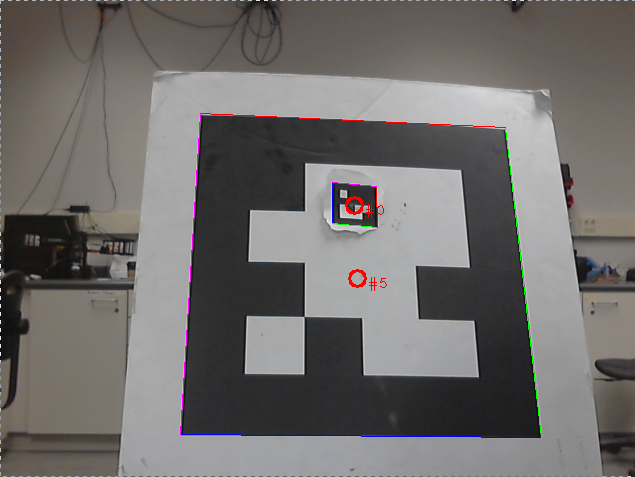
\includegraphics[width=\textwidth]{images/apriltags_1.png}
		\caption{2 Apriltags Detected}
	\end{subfigure}
	\begin{subfigure}[b]{0.45\linewidth}
		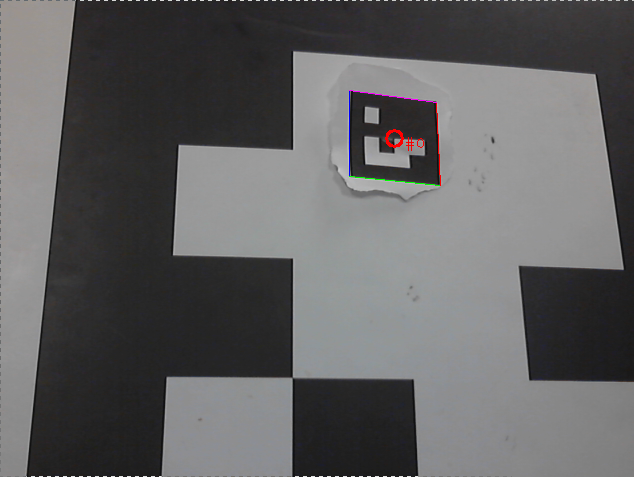
\includegraphics[width=\textwidth]{images/apriltags_3.png}
		\caption{1 Apriltag Detected }
	\end{subfigure}
	\caption{Apriltag Inception - To mitigate the FOV problem}
	\label{fig:apriltag}
\end{figure}

On the landing target from we have successfully calibrated the logitech webcam and used the Apriltag library to obtain a pose estimate, and have manually verified the estimates are accurate, for distance the error is $\pm 1$cm. We have also successfully implemented the ability to identify two different apriltags of different sizes (see Fig~\ref{fig:apriltag}), pose estimates from both apriltags are equal.

Next is to workout how to transform the measurements from the pose estimates of the apriltags in relation to the quadrotor's body frame.



\subsubsubsection{Detection Delay}

\begin{equation}
    t_{\text{capture}} = t - \delta t_{\text{camera}} + \delta t_{detection}
\end{equation}




\bibliography{report}{}
\bibliographystyle{ieeetr}

\end{document}
